\documentclass[12pt]{article}

\usepackage[utf8]{inputenc}
\usepackage[czech]{babel}
\usepackage{a4wide}
\usepackage{graphicx}
\linespread{1.3}

\usepackage{fancyhdr}
\pagestyle{fancy}
\fancyhf{}

\renewcommand{\headrulewidth}{0.4pt}
\renewcommand{\footrulewidth}{0.4pt}

% Nastaveni hlavicky a paticky.
\lhead{X33EJA - Enterprise Java}
\rhead{Tomáš Čerevka, Adam Činčura}
\lfoot{\today}
\rfoot{\thepage}

\begin{document}

\begin{Huge}Bookcase - checkpoint 1\end{Huge}

\section{Motivace}

Již od dob vynalezení knihtisku byly knihy shromažďovány - nejdříve do soukromých sbírek, pak do veřejných knihoven. Dnes již není žádnou vzácností, když lidé mají doma svou vlastní malou knihovnu. Lidé si knihy mezi sebou často půjčují, přičemž svým známým důvěřují, že jim knihu zase po čase vrátí. Leckdy se ale stává, že některý ze zúčastněných na zápůjčku zapomene, ať již neúmyslně či zcela záměrně, a kniha tak změní svou knihovnu. Tak vzniká potřeba vytvořit systém, který umožní široké veřejnosti evidenci své knihovny včetně systému zápůjček a rezervací.

\section{Uživatelé}

Systém bude určen hlavně pro dva druhy uživatelů, přičemž se nevylučuje možnost vystupovat v obou rolích zároveň.

\subsection{Knihovník}

Knihovníkovi systém umožní správu jeho osobní knihovny. Má možnost třídit s knihy do poliček, přičemž každý svazek může být zařazen ve více poličkách. Dále si může dělat poznámky k jednotlivým výtiskům a označovat ty, které jsou aktuálně zapůjčeny. Knihovník si vede seznam čtenářů, u kterých si eviduje zápůjčky. 

\subsection{Čtenář}

Čtenář má možnost kontrolovat si zapůjčky, které má vedeny u jednotlivých knihovníků. Nabízí se mu také možnost procházení knihoven, do nichž má přístup, a zarezervování si knihy. Aby čtenář získal přístup do knihovny, musí o něj požádat a knihovník mu ho musí udělit.

\section{Funkce}

Systém umožní:

\begin{itemize}
	\item registraci uživatele.
	\item vedení vlastní knihovny.
	\item evidenci zápůjček.
	\item zasílání upomínek e-mailem.
	\item procházení knihoven, v nichž je uživatel schválen.
\end{itemize}

\section{Omezení}

Jelikož systém vychází z předpokladu, že knihovník a čtenář se znají a knihu si půjčují ze známosti, nebude k dispozici možnost procházení všech knihoven. Čtenář bude mít k dispozici jen ty knihovny, v nichž je zaregistrován.

\section{ER model}

Diagram s ER modelem na obrázku \ref{er} zachycuje jednotlivé entity v systému a vztahy mezi nimi dle popisu výše.

\begin{figure}
	\centering
	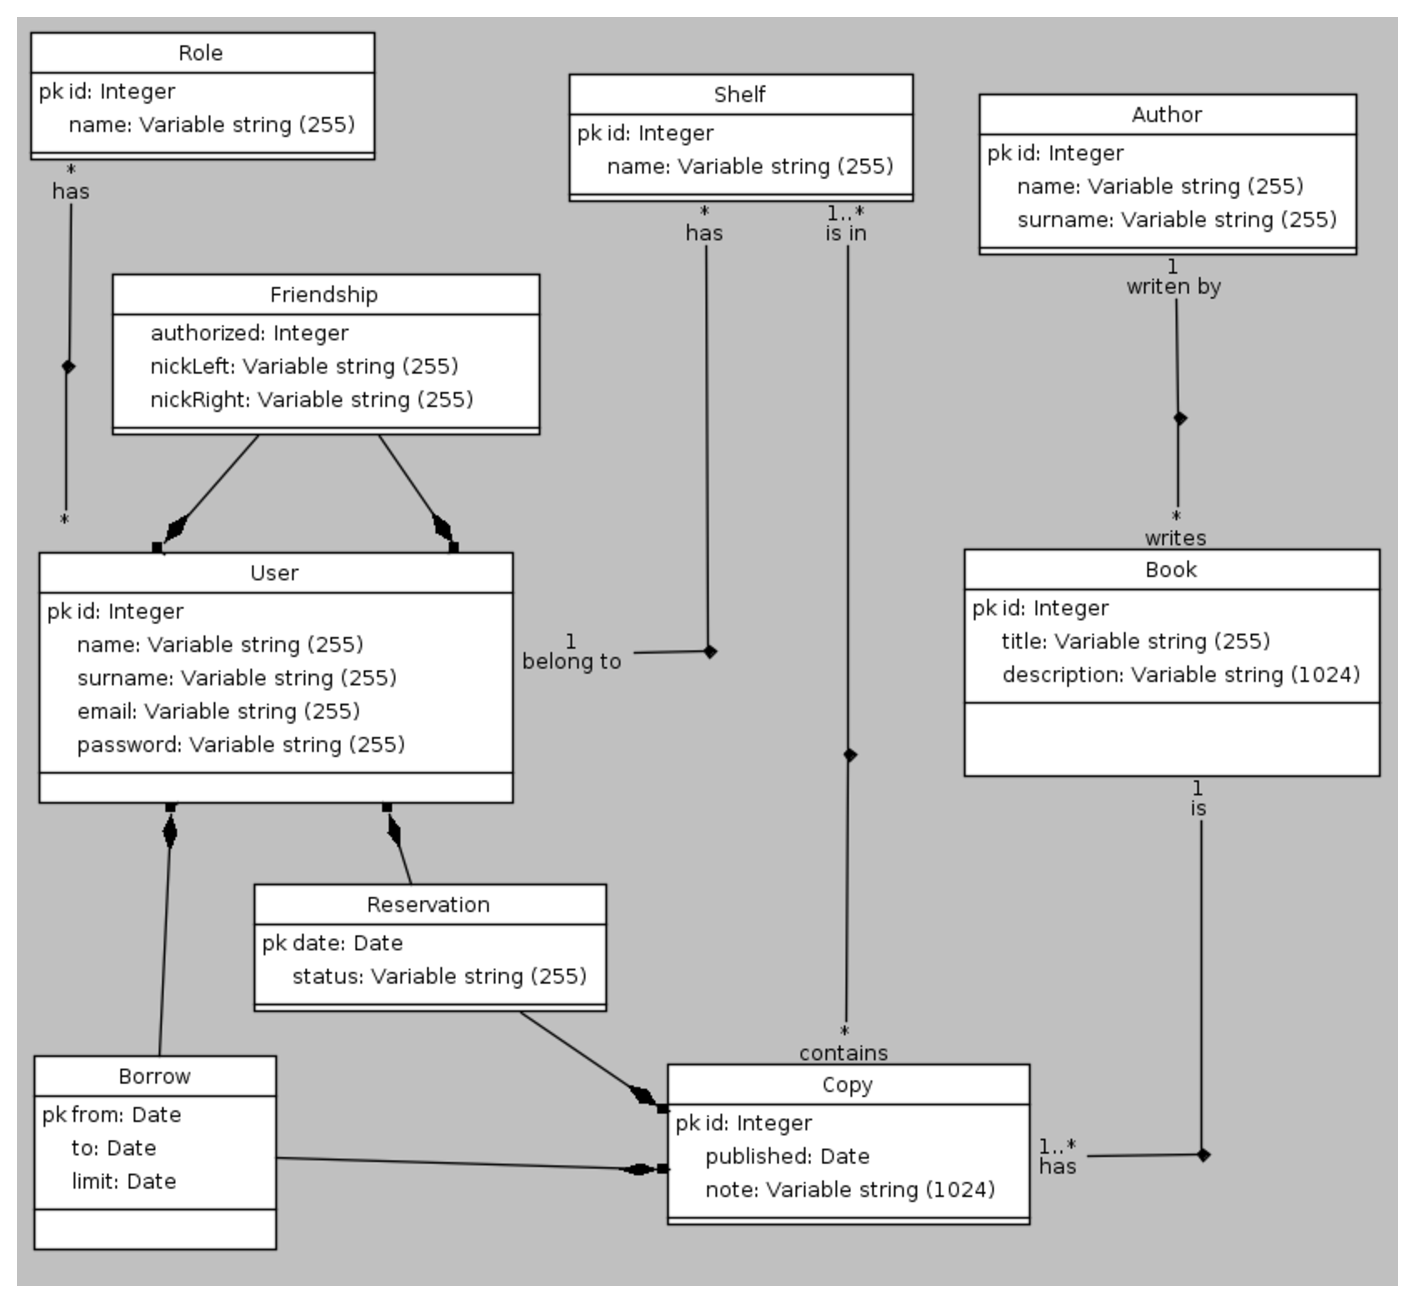
\includegraphics[scale=0.7]{model.eps}
	\caption{ER model}
	\label{er}
\end{figure}

\end{document}
